
\documentclass[nooutcomes]{ximera}
%\documentclass[space,handout,nooutcomes]{ximera}

% For preamble materials

\graphicspath{
  {./}
  {algorithms/}
  {../algorithms/}
}


%%% This set of code is all of our user defined commands
\newcommand{\bysame}{\mbox{\rule{3em}{.4pt}}\,}
\newcommand{\N}{\mathbb N}
\newcommand{\C}{\mathbb C}
\newcommand{\W}{\mathbb W}
\newcommand{\Z}{\mathbb Z}
\newcommand{\Q}{\mathbb Q}
\newcommand{\R}{\mathbb R}
\newcommand{\A}{\mathbb A}
\newcommand{\D}{\mathcal D}
\newcommand{\F}{\mathcal F}
\newcommand{\ph}{\varphi}
\newcommand{\ep}{\varepsilon}
\newcommand{\aph}{\alpha}
\newcommand{\QM}{\begin{center}{\huge\textbf{?}}\end{center}}

\renewcommand{\le}{\leqslant}
\renewcommand{\ge}{\geqslant}
\renewcommand{\a}{\wedge}
\renewcommand{\v}{\vee}
\renewcommand{\l}{\ell}
\newcommand{\mat}{\mathsf}
\renewcommand{\vec}{\mathbf}
\renewcommand{\subset}{\subseteq}
\renewcommand{\supset}{\supseteq}
\renewcommand{\emptyset}{\varnothing}
\newcommand{\xto}{\xrightarrow}
\renewcommand{\qedsymbol}{$\blacksquare$}
\newcommand{\bibname}{References and Further Reading}
\renewcommand{\bar}{\protect\overline}
\renewcommand{\hat}{\protect\widehat}
\renewcommand{\tilde}{\widetilde}
\newcommand{\tri}{\triangle}
\newcommand{\minipad}{\vspace{1ex}}
\newcommand{\leftexp}[2]{{\vphantom{#2}}^{#1}{#2}}

%% More user defined commands
\renewcommand{\epsilon}{\varepsilon}
\renewcommand{\theta}{\vartheta} %% only for kmath
\renewcommand{\l}{\ell}
\renewcommand{\d}{\, d}
\newcommand{\ddx}{\frac{d}{dx}}
\newcommand{\dydx}{\frac{dy}{dx}}


\usepackage{bigstrut}


\newenvironment{sectionOutcomes}{}{}

\usepackage{array}
%\setlength{\extrarowheight}{-.2cm}   % Commented out by Findell to fix table headings.  Was this for typesetting division?  
\newdimen\digitwidth
\settowidth\digitwidth{9}
\def~{\hspace{\digitwidth}}
\def\divrule#1#2{
\noalign{\moveright#1\digitwidth
\vbox{\hrule width#2\digitwidth}}}


\title{Integers}
\author{Bart Snapp and Brad Findell and Jenny Sheldon}
\begin{document}
\begin{abstract}
Problems about integers.
\end{abstract}
\maketitle


%\begin{problem}
%Problem
%\begin{freeResponse}
%\begin{hint}
%Hint
%\end{hint}
%\end{freeResponse}
%\end{problem} 


\begin{problem}
Describe the set of integers. Give some relevant and revealing
  examples/nonexamples.
\begin{freeResponse}
\begin{hint}
The integers are the counting numbers, 0, and the opposites of the counting numbers.  
\[\{ \dots, -3, -2, -1, 0, 1, 2, 3, \dots\}\]
\end{hint}
\end{freeResponse}
\end{problem}

\begin{problem}
Give some examples of contexts we might use to describe integers. What relevant properties should your context have?
\begin{freeResponse}
\begin{hint}
Common contexts include temperature, bank balance, and elevation.  A good context should have a sense of positive and negative, or a quantity and its opposite.
\end{hint}
\end{freeResponse}
\end{problem}

For the next few problems, identify which operation should be used to solve the problem.

\begin{problem}
Alison has $34$ head bands.  April has $38$ headbands.  How many more headbands does April have?
\begin{prompt}
The problem above is an example of:
\begin{multipleChoice}
\choice{Addition.}
\choice{Take-away subtraction.}
\choice[correct]{Comparison subtraction.}
\choice{Missing-addend subtraction.}
\end{multipleChoice}
\end{prompt}
\end{problem}


\begin{problem}
Gabe has a bank balance of $\$17$.  After he spends $\$22$, what will Gabe's balance be?
\begin{prompt}
The problem above is an example of:
\begin{multipleChoice}
\choice{Addition.}
\choice[correct]{Take-away subtraction.}
\choice{Comparison subtraction.}
\choice{Missing-addend subtraction.}
\end{multipleChoice}
\end{prompt}
\end{problem}


\begin{problem}
Yesterday, Ollie was $9$ miles west of home.  Today, Ollie is $6$ miles east of home.  How far did Ollie travel overnight?
\begin{prompt}
The problem above is an example of:
\begin{multipleChoice}
\choice{Addition.}
\choice{Take-away subtraction.}
\choice{Comparison subtraction.}
\choice[correct]{Missing-addend subtraction.}
\end{multipleChoice}
\end{prompt}
\begin{hint}
The problem is asking what was added to Ollie's distance from home yesterday in order to get to today's location.
\end{hint}
\end{problem}


\begin{problem}
Last week, the average temperature was $-2$ degrees Celsius.  This week, the average temperature is $4$ degrees warmer.  What is the average temperature this week?
\begin{prompt}
The problem above is an example of:
\begin{multipleChoice}
\choice[correct]{Addition.}
\choice{Take-away subtraction.}
\choice{Comparison subtraction.}
\choice{Missing-addend subtraction.}
\end{multipleChoice}
\end{prompt}
\end{problem}


The next few problems use the red and black chips we discussed for modeling integers.

\begin{problem}
What is the total value of the chips in the following picture?
\begin{center} 
\begin{tikzpicture}
	\draw[red, fill=red](0,0) circle (0.5cm);
	\draw[red, fill=red] (2,0) circle (0.5cm);
	\draw[red, fill=red] (4,0) circle (0.5cm);
	\draw[black, fill=black] (6,0) circle (0.5cm);
	\draw[black, fill=black] (8,0) circle (0.5cm);
	\draw[black, fill=black] (10,0) circle (0.5cm);
	\draw[black, fill=black] (12,0) circle (0.5cm);
\end{tikzpicture} \end{center}

\begin{prompt}
The total value is $\answer[given]{1}$.
\end{prompt}

\end{problem}

\begin{question}
What is the total value of all of the chips in the picture below?
\begin{center}

\begin{tikzpicture}
\draw[black, fill=black](0,0) circle (0.5cm);
\draw[black, fill=black](2,0) circle (0.5cm);
\draw[black, fill=black](4,0) circle (0.5cm);
\draw[black, fill=black](6,0) circle (0.5cm);
\draw[red, fill=red] (6, 2) circle (0.5cm);
\draw[red, fill=red] (4, 2) circle (0.5cm);
\end{tikzpicture}
\end{center}
The total value of the chips is $\answer[given]{2}$.
\end{question}

\begin{question}
Suppose you would like to use chips to represent a total value of $8$.  Which of the following combinations of chips would give you this value?
\begin{selectAll}
\choice[correct]{$8$ black chips}
\choice{$8$ red chips}
\choice[correct]{$10$ black chips and $2$ red chips}
\choice{$2$ black chips and $10$ red chips}
\choice[correct]{$24$ black chips and $16$ red chips}
\choice{$3$ black chips and $11$ red chips}
\choice{$5$ black chips and $3$ red chips}
\end{selectAll}
\end{question}


\begin{question}
Suppose you would like to use chips to represent a total value of $-6$.  Which of the following combinations of chips would give you this value?
\begin{selectAll}
\choice{$-6$ black chips}
\choice[correct]{$6$ red chips}
\choice{$6$ black chips and $6$ red chips}
\choice{$2$ black chips and $4$ red chips}
\choice{$10$ black chips and $6$ red chips}
\choice[correct]{$24$ black chips and $30$ red chips}
\choice{$18$ black chips and $12$ red chips}
\end{selectAll}
\end{question}


\begin{question}
You are working on the subtraction problem $10 - (-2)$, and you would like to solve this problem using red and black chips from a take-away perspective.  First, you put your chips down on the table.  What chips will you need?

\begin{prompt}
You need to model a total value of $\answer[given]{10}$ using the chips.  You will need at least $\answer[given]{2}$ red chips in your model so that you have enough to take away.
\end{prompt}
\begin{question}
You decide to use a model with $12$ black chips and $2$ red chips.  How many chips do you take away, and what is left?

\begin{prompt}
You take away $\answer[given]{2}$ \wordChoice{\choice{black}\choice[correct]{red}} chips, leaving $\answer[given]{12}$ black chips and $\answer[given]{0}$ red chips.
\end{prompt}
\begin{question}
What is $10 - (-2)$, from your result with the chips?

\begin{prompt}
$10 - (-2) = \answer[given]{12}$
\end{prompt}
\end{question}
\end{question}
\end{question}


\begin{question}
You are working on the subtraction problem $(-4) - (-7)$, and you would like to solve this problem using red and black chips from a take-away perspective.  First, you put your chips down on the table.  What chips will you need?

\begin{prompt}
You need to model a total value of $\answer[given]{-4}$ using the chips.  You will need at least $\answer[given]{7}$ red chips in your model so that you have enough to take away.
\end{prompt}

\begin{question}
You decide to use a model with $6$ black chips and $10$ red chips.  How many chips do you take away, and what is left?

\begin{prompt}
You take away $\answer[given]{7}$ \wordChoice{\choice{black}\choice[correct]{red}} chips, leaving $\answer[given]{6}$ black chips and $\answer[given]{3}$ red chips.
\end{prompt}

\begin{question}
What is $(-4) - (-7)$, from your result with the chips?

\begin{prompt}
$(-4) - (-7) = \answer[given]{3}$
\end{prompt}
\end{question}
\end{question}
\end{question}



\begin{question}
You are working on the subtraction problem $1-5$, and you would like to solve this problem using red and black chips from a missing-addend perspective.  First, you change your problem into the related addition problem.  What is the result?

\begin{prompt}
The related addition problem is $\answer[given]{1} = \answer[given]{5} + ?$.
\end{prompt}
\begin{question}
 We now need to begin with a model for $5$ and decide how to get to $1$.  What chips would we lay down to do this?

\begin{prompt}
	We lay down $\answer[given]{4}$ \wordChoice{\choice{black} \choice[correct]{red}} chips.
\end{prompt}
\begin{question}
 Using our work with the chips, what is $1-5$?
 
 \begin{prompt}
 	$1-5 = \answer[given]{-4}$
 \end{prompt}
\end{question}
\end{question}
\end{question}




\begin{question}
You are working on the subtraction problem $(-8)-7$, and you would like to solve this problem using red and black chips from a missing-addend perspective.  First, you change your problem into the related addition problem.  What is the result?

\begin{prompt}
The related addition problem is $\answer[given]{-8} = \answer[given]{7} + ?$.
\end{prompt}
\begin{question}
 We now need to begin with a model for $7$ and decide how to get to $-8$.  What chips would we lay down to do this?

\begin{prompt}
	We lay down $\answer[given]{15}$ \wordChoice{\choice{black} \choice[correct]{red}} chips.
\end{prompt}
\begin{question}
 Using our work with the chips, what is $(-8)-7$?
 
 \begin{prompt}
 	$(-8)-7 = \answer[given]{-15}$
 \end{prompt}
\end{question}
\end{question}
\end{question}


\begin{question}
In the picture below, use our definition of multiplication to find the total value of the chips.
\begin{center}
\begin{tikzpicture}
\draw[red,fill=red] (0,0) circle (0.4cm);
\draw[red,fill=red] (1,0) circle (0.4cm);
\draw[red, fill=red] (0,1) circle (0.4cm);
\draw[red, fill=red] (1,1) circle (0.4cm);
\draw[red,fill=red] (4,0) circle (0.4cm);
\draw[red,fill=red] (5,0) circle (0.4cm);
\draw[red, fill=red] (4,1) circle (0.4cm);
\draw[red, fill=red] (5,1) circle (0.4cm);
\draw[red,fill=red] (8,0) circle (0.4cm);
\draw[red,fill=red] (9,0) circle (0.4cm);
\draw[red, fill=red] (8,1) circle (0.4cm);
\draw[red, fill=red] (9,1) circle (0.4cm);
\end{tikzpicture}\end{center}

\begin{prompt}
The total value of the chips is $\answer[given]{3} \times \answer[given]{-4}$.
\end{prompt}
\end{question}


\begin{example}
Imagine using a number line like the one below to solve the subtraction problem $-8 - 4$.
\begin{center}
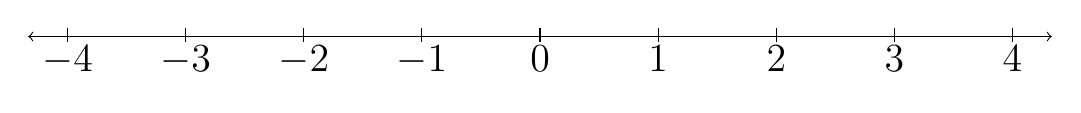
\begin{tikzpicture}[font=\Large]
\draw[<->] (-0.5,0) -- (12.5,0);
\foreach \x in {0,1.5, 3, 4.5, 6, 7.5, 9, 10.5,12}
\draw[shift={(\x,0)},color=black] (0pt,3pt) -- (0pt,-2pt);
\draw (0,0) node[below]{$-4$};
\draw (1.5,0) node[below]{$-3$};
\draw (3,0) node[below]{$-2$};
\draw (4.5,0) node[below]{$-1$};
\draw (6,0) node[below]{$0$};
\draw (7.5,0) node[below]{$1$};
\draw (9,0) node[below]{$2$};
\draw (10.5,0) node[below]{$3$};
\draw (12,0) node[below]{$4$};
\end{tikzpicture}  
\end{center}
We begin by standing on the number line at the tick marked with $\answer[given]{-8}$.  Since 
we are subtracting, we face towards the \wordChoice{\choice{right} \choice[correct]{left}}.  We 
will move $\answer[given]{4}$ spaces \wordChoice{\choice[correct]{forward} \choice{backward}}, 
since $4$ is positive.  Where on the number line are we now? 

\begin{prompt}
We are located at the tick labeled $\answer[given]{-12}$.
\end{prompt}
\end{example}

\begin{example}
Imagine using a number line like the one below to solve the subtraction problem $(-22) - (-54)$.
\begin{center}
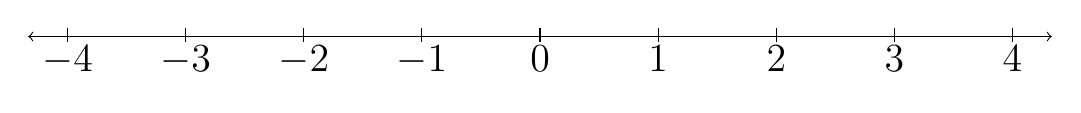
\begin{tikzpicture}[font=\Large]
\draw[<->] (-0.5,0) -- (12.5,0);
\foreach \x in {0,1.5, 3, 4.5, 6, 7.5, 9, 10.5,12}
\draw[shift={(\x,0)},color=black] (0pt,3pt) -- (0pt,-2pt);
\draw (0,0) node[below]{$-4$};
\draw (1.5,0) node[below]{$-3$};
\draw (3,0) node[below]{$-2$};
\draw (4.5,0) node[below]{$-1$};
\draw (6,0) node[below]{$0$};
\draw (7.5,0) node[below]{$1$};
\draw (9,0) node[below]{$2$};
\draw (10.5,0) node[below]{$3$};
\draw (12,0) node[below]{$4$};
\end{tikzpicture}  
\end{center}
We begin by standing on the number line at the tick marked with $\answer[given]{-22}$.  Since 
we are subtracting, we face towards the \wordChoice{\choice{right} \choice[correct]{left}}.  We will 
move $\answer[given]{54}$ spaces \wordChoice{\choice{forward} \choice[correct]{backward}}, since 
$54$ is negative.  Where on the number line are we now? 

\begin{prompt}
We are located at the tick labeled $\answer[given]{32}$.
\end{prompt}
\end{example}


\begin{question}
In your own words, what is the difference between subtraction and negation?
\begin{freeResponse}
\begin{hint}
Subtraction is an operation, requiring two numbers.  With subtraction, we have two quantities that we are trying to relate.  With our models, subtraction requires some movement: removing chips, adding chips, or walking on the number line.  Negation, on the other hand, only requires a single value.  With negation, we are essentially just asking, ``What is the opposite?''  With our models, this is essentially a switching rather than a moving: we switch from black chips to red, or we face backward instead of forward.
\end{hint}
\end{freeResponse}
\end{question}








\end{document}